\chapter{Koding Tingkat Medium}
Pada bagian ini akan dibahas berbagai pemrograman Python yang lebih {\em advanced}. 
Sebetulnya yang akan dibahas adalah contoh-contoh kode Python dengan menggunakan 
berbagai paket yang tersedia.

\section{Argumen CLI}
Seringkali kita harus membuat sebuah program dalam bentuk {\em command line interface}
(CLI) yang kemudian membaca argumen yang diberikan. 
Misalnya kita ingin program kita memproses sebuah berkas yang namanya kita
berikan di {\em command line}.

\begin{verbatim}
$ program filename.pdf
\end{verbatim}

Apa yang kita berikan kepada program di atas disebut {\em argument}.
Pada contoh di atas, {\em argument}-nya adalah ``filename.pdf''.
Program kita harus dapat membaca {\em argument} yang kita berikan kepada program
tersebut. Bagaimana caranya? Ada banyak caranya. Salah satunya dicontohkan
pada contoh berikut ini.

\begin{verbatim}
# contoh parsing argumen yang diberikan kepada program
# beri nama skrip ini cli-args.py
# cara menjalankan:
#    python3 cli-args.py opsi1 opsi2 opsi3 
# opsi bisa banyak

import sys
# periksa jumlah argumennya

numberargs = len(sys.argv)
# tanpa argumen, hasilnya akan 0 (nol)
# nama skrip adalah sys.argv[0]

# print argumen yang diberikan
for i in range(numberargs):
   print(i, sys.argv[i])
\end{verbatim}}

Dari contoh tersebut, Anda dapat mengembangkan hal-hal yang lain.
Misalnya Anda ingin memastikan bahwa program Anda mendapatkan {\em argument}
dalam jumlah yang cukup (misalnya harus 3). Jika argumen yang diberikan kurang,
maka dia akan memberikan petunjuk cara penggunaan skrip (program) kita
dan kemudian keluar (dengan exit).
(Catatan: biasanya {\em exit} memiliki nilai tidak nol kalau ada kesalahan.
Kalau keluar normal, angkanya nol.)

\begin{verbatim}
if (numberargs) < 4:
   print("Usage: " + sys.argv[0] + " data1 data2 data3")
exit(1)
    
\end{verbatim}

\section{Numpy}
Numpy adalah paket python untuk berbagai aplikasi {\em scientific}.
Di dalamnya ada {\em N-dimensional object}, {\em linear algebra},
{\em Fourier transform}, dan seterusnya.
Sebagai contoh, jika kita ingin membangkitkan bilangan random dengan 
distribusi tertentu (uniform atau normal), maka kita dapat menggunakan 
paket Numpy ini.
Biasanya paket Numpy ini sudah terpasang ketika kita memasang Python,
tetapi jika belum terpasang maka modul Numpy ini dapat kita pasang sendiri.

\begin{verbatim}
$ sudo pip install numpy
\end{verbatim}

Contoh-contoh penggunaan paket Numpy akan digabungkan dengan bagian lain.
Berikut ini adalah contoh sederhana penggunaan dari Numpy.

\begin{verbatim}
>>> import numpy as np
>>> a = np.arange(15).reshape(3, 5)
>>> a
array([[ 0,  1,  2,  3,  4],
       [ 5,  6,  7,  8,  9],
       [10, 11, 12, 13, 14]])
\end{verbatim}

\section{Matlplotlib}
Salah satu aplikasi yang cukup sering dibutuhkan ketika kita membuat program 
untuk keperluan penelitian adalah membuat grafik (plot). 
Salah satu {\em library} yang baik untuk digunakan adalah {\em matplotlib}. 
Paket ini membutuhkan paket lain, yaitu {\em python-tk}. 
Untuk itu python-tk ini harus dipasang dulu. 
Di bawah ini adalah contoh pemasangan python-tk di sistem Linux (berbasis Debian) 
dengan menggunakan perintah apt-get.

\begin{verbatim}
$ sudo apt-get install python-tk
$ sudo pip install matplotlib
\end{verbatim}

Berikut ini adalah sebuah contoh penggunaan Matplotlib dan Numpy. Pada contoh ini kita akan membuat kumpulan data yang memiliki karakteristik ``sekitar'' persamaan 
$Y = Ax + b$.
Untuk itu perlu dihasilkan data yang sudah ditambahi atau dikurangi dengan angka random (yang dibuat dengan menggunakan Numpy). (Kode ini diambil dari buku ``Getting Started with Tensorflow''\cite{tensorflowstarted}.)
Hasilnya dapat dilihat pada gambar~\ref{fig:randomnumpy}


\begin{verbatim}
import numpy as np
import matplotlib.pyplot as plt

# persamaan y = a*x + b
a = 0.25
b = 0.75
jumlah_titik = 300

# buat dua list yang masih kosong
x_point = []
y_point = []

for i in range(jumlah_titik):
    x = np.random.normal(0.0,0.4)
    y = a*x + b + np.random.normal(0.0,0.1)
    x_point.append([x])
    y_point.append([y])

plt.plot(x_point,y_point,'o',label='Random Data')
plt.legend()
plt.show()
\end{verbatim}


\begin{figure}[ht]
\fbox{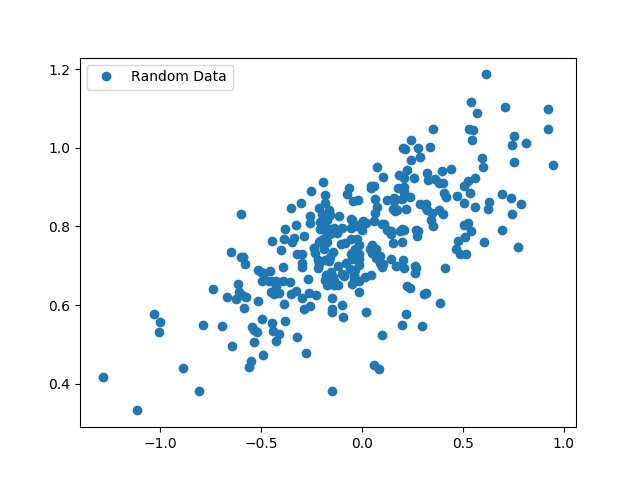
\includegraphics[width=1.0\linewidth]{graphics/random-data.png}}
\caption{Contoh Pembangkitan Random Data}
\label{fig:randomnumpy}
\end{figure}

Jika kode di atas ingin dijalankan di dalam {\em Jupyter Notebook},
maka baris pertama perlu ditambahkan ini:

\begin{verbatim}
%matplotlib notebook
\end{verbatim}

Data ($x$ dan $y$) pada contoh di atas dapat disimpan (diekspor) ke berkas
dalam format CSV ({\em comma separated value}) dengan menggunakan Numpy
seperti contoh di bawah ini.
Berkas ``linear-regression.csv'' disimpan pada direktori dimana kode
ini dijalankan. Variabel $x\_point$ dan $y\_point$ akan dimasukkan ke
berkas tersebut dengan format yang didefinisikan dalam {\em fmt}.
Pada contoh di bawah ini format yang akan digunakan adalah 
{\em floating point} dengan 5 digit di belakang koma.
Variabel tersebut dipisahkan dengan menggunakan koma (,) sebagaimana
dijabarkan dalam {\em delimiter}.

\begin{verbatim}
np.savetxt("linear-regression.csv", np.column_stack([x_point, y_point]), fmt='%.5f', delimiter=', ')
\end{verbatim}

Data di atas dapat dibaca kembali dari berkas CSV dan dilakukan
perhitungan ({\em linear regression}) untuk mencari faktor {\em gradient}
(faktor $A$) dan $b$ dalam persamaan $Y = a*x + b$.
Perhitungan ini membutuhkan modul {\em Scipy} yang harus dipasang
secara terpisah. (Gunakan pip untuk memasang modul scipy itu.)

\begin{verbatim}
#read CSV of data and calculate a and b
# y = ax + b
import numpy as np
# do not forget to install scipy first: python3 -m pip install scipy
from scipy import stats

my_csv = np.genfromtxt('linear-regression.csv', delimiter=',')
xp, yp = my_csv.transpose()
gradient,intercept,r_value,p_value,std_err=stats.linregress(xp,yp)
print("Gradient and intercept",gradient,intercept)
print("R-squared",r_value**2)
print("p-value",p_value)
\end{verbatim}

Jika diperlukan, data tersebut dapat ditampilkan ulang dan garis (lurus)
dapat digambarkan pula.

\section{Pandas}
Pandas adalah library untuk data processing. Dia banyak digunakan untuk
berbagai aplikasi, seperti misalnya di Machine Learning.

Langkah pertama yang dilakukan adalah memasang Pandas.

\begin{verbatim}
$ sudo pip install pandas
\end{verbatim}

Jika Anda menggunakan Python3, maka gunakan perintah berikut.
\begin{verbatim}
$ sudo python3 -m pip install pandas
\end{verbatim}

Setelah Pandas terpasang, mari kita coba membuat sebuat {\em Series}.
Kali ini dia berisi data bilangan dan $NaN$.
Pandas akan secara otomatis membuat indeks dari data tersebut (dengan
index bilangan integer)\footnote{Contoh lain dapat dilihat di
https://pandas.pydata.org/pandas-docs/stable/10min.html}.

\begin{verbatim}
import pandas as pd
import numpy as np
import matplotlib.pyplot as plt

# create series
ser = pd.Series([1,3,5,7,np.nan,9,11])
print(ser)
\end{verbatim}

Hasilnya adalah sebagai berikut.
\begin{verbatim}
0     1.0
1     3.0
2     5.0
3     7.0
4     NaN
5     9.0
6    11.0
dtype: float64
\end{verbatim}


\section{Kriptografi}
Sebagaimana bidang lain, Python memiliki {\em library} yang lengkap untuk
kriptografi. Berikut ini hanya beberapa contoh penggunaan {\em library}
tersebut.

\subsection{Fungsi Hash}
Fungsi hash adalah fungsi satu arah yang memberikan tanda ({\em signature})
dari data digital; {\em stream of data} dan berkas.
Perubahan satu bit saja dari data tersebut akan mengubah nilai dari
{\em hash} yang dihasilkan. Itulah sebabnya fungsi {\em hash} dapat
digunakan untuk menjamin integritas data.

Ada banyak algoritma fungsi hash. Algoritma yang terkenal adalah MD5
dan SHA. Saat ini MD5 sudah dianggap tidak layak lagi karena sudah
ditemukan {\em collision}, yaitu nilai {\em hash} yang sama untuk data
yang berbeda. SHA~256 merupakan algoritma yang dianggap cocok saat ini.

\begin{verbatim}
unix$ echo "beli 10000" | shasum -a 256
375a6c46228994656932f4aa17d9ae50f21da75a31ff17f8517c255c06cba809 -

unix$ cat pesan1.txt
beli 10000
unix$ shasum -a 256 pesan1.txt
375a6c46228994656932f4aa17d9ae50f21da75a31ff17f8517c255c06cba809 pesan1.txt

unix$ cat pesan2.txt
beli 1000
unix$ shasum -a 256 pesan2.txt
5901bccc6a0556fac2b4a164ef831a7ed4ceddeb60c6ddde1162f5a40b9d2917 pesan2.txt
\end{verbatim}

Contoh kode Python untuk hal di atas adalah sebagai berikut:

\begin{verbatim}
# Contoh fungsi hash
import hashlib
h = hashlib.sha256("beli 10000\n")
print h.hexdigest()
\end{verbatim}


Salah satu pemanfaatan ``baru'' dari fungsi {\em hash} ini adalah pada
algoritma {\em Blockchain} yang digunakan pada {\em Bitcoin}. Sedikit
cerita tentang hal ini ada di blog
saya~\footnote{https://rahard.wordpress.com/2018/03/10/berburu-hash/}.
